\documentclass{standalone}
\begin{document}
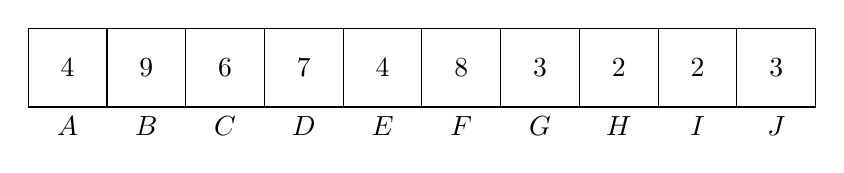
\begin{tikzpicture}

\draw (0, 0) -- (10, 0);
\draw (0, 1) -- (10, 1);
\foreach \i in {0,...,10}
{
    \draw (\i,0) -- (\i, 1);
}

\draw ( 0.5, 0) node[below]{$A$};
\draw ( 1.5, 0) node[below]{$B$};
\draw ( 2.5, 0) node[below]{$C$};
\draw ( 3.5, 0) node[below]{$D$};
\draw ( 4.5, 0) node[below]{$E$};

\draw ( 5.5, 0) node[below]{$F$};
\draw ( 6.5, 0) node[below]{$G$};
\draw ( 7.5, 0) node[below]{$H$};
\draw ( 8.5, 0) node[below]{$I$};
\draw ( 9.5, 0) node[below]{$J$};

% grid indices
\draw ( 0.5, .5) node[]{$4$};
\draw ( 1.5, .5) node[]{$9$};
\draw ( 2.5, .5) node[]{$6$};
\draw ( 3.5, .5) node[]{$7$};
\draw ( 4.5, .5) node[]{$4$};

\draw ( 5.5, .5) node[]{$8$};
\draw ( 6.5, .5) node[]{$3$};
\draw ( 7.5, .5) node[]{$2$};
\draw ( 8.5, .5) node[]{$2$};
\draw ( 9.5, .5) node[]{$3$};

\end{tikzpicture}
\end{document}
